\section{OpenPRA Web-App Architecture}
The system consists of a web-based front end, a standardized OpenPRA \acrfull{mef} schema, a back end providing \acrfull{rest}ful \acrfull{api}s, distributed databases, and a distributed job queue, as shown in figure \ref{fig:openpra_overview}. Each layer has a distinct role:

\begin{figure}[h!]
  \centering
  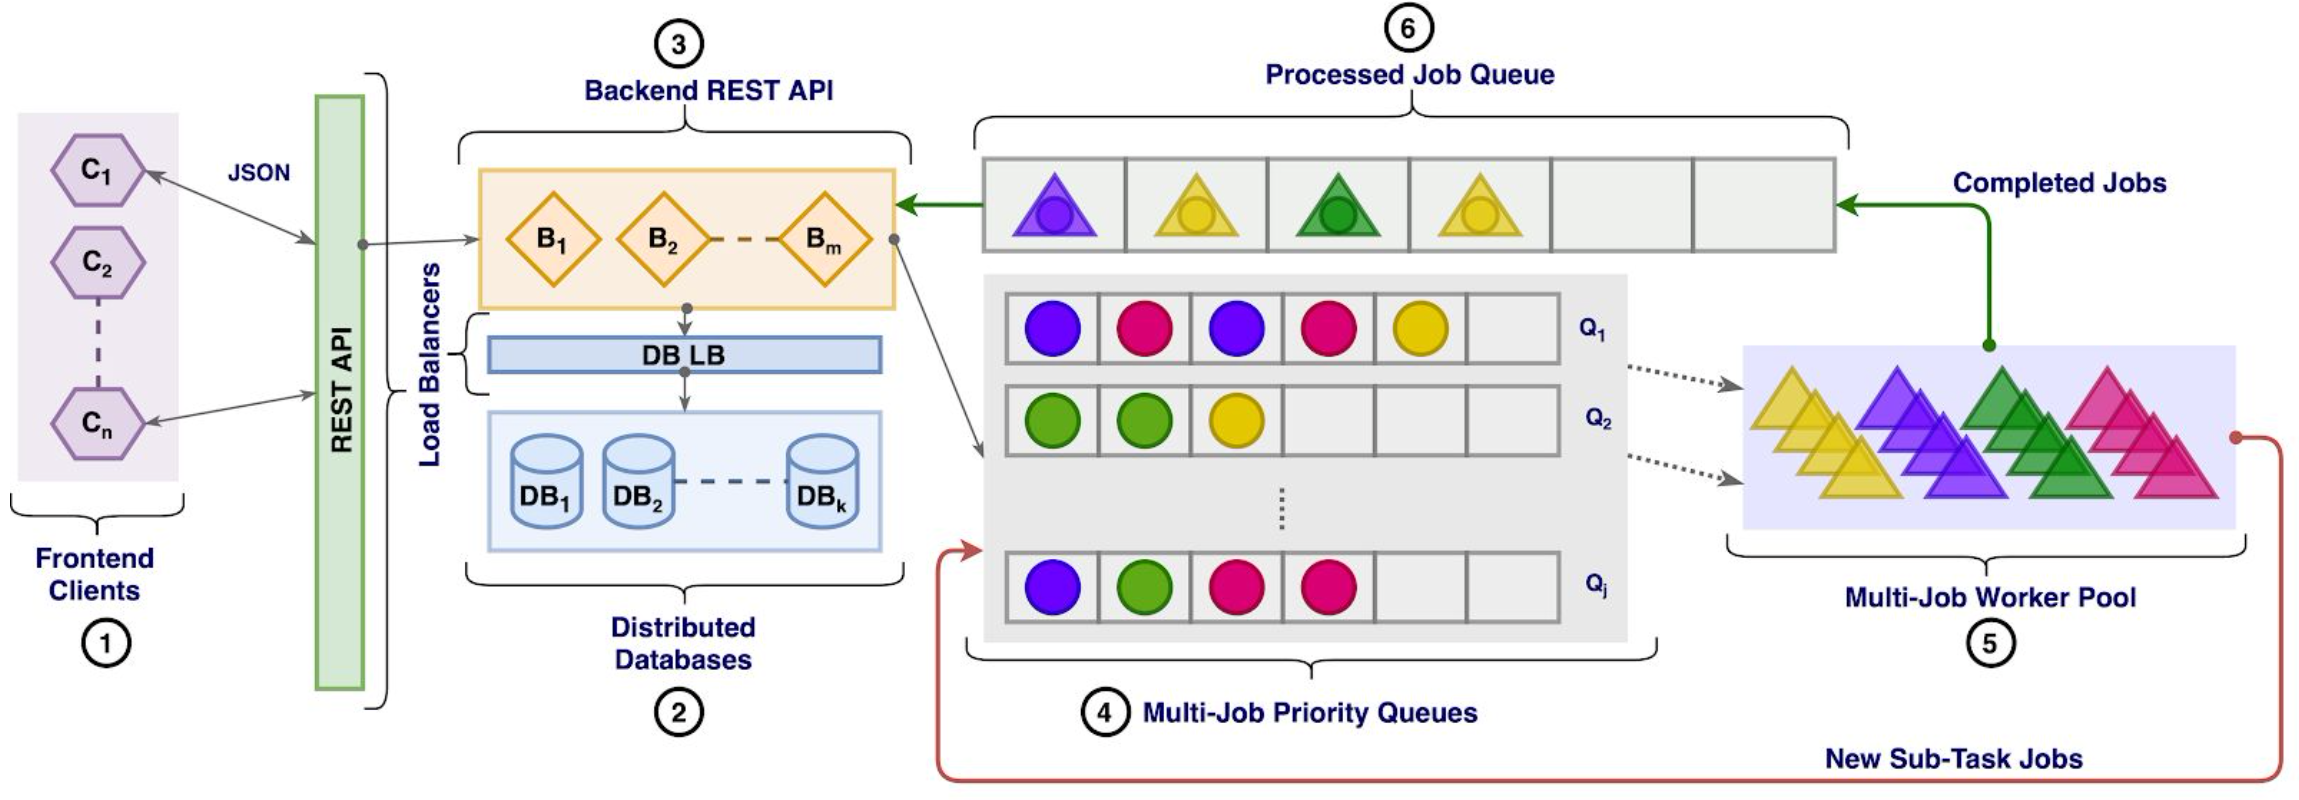
\includegraphics[width=0.9\textwidth]{4_proposed_solution/web_app/figures/openpra_overview.png}
  \caption{High-level functional overview of the framework.}
  \label{fig:openpra_overview}
\end{figure}

\begin{itemize}
\item \textbf{Front-end (Web \acrshort{ui})}: Provides a user interface for editing \acrshort{pra} models, configuring solver parameters and for visualizing analysis results. Figure \ref{fig:landing_page} shows the landing page of the web app.
\item \textbf{OpenPRA \acrshort{mef} schemas}: Defines a common \acrshort{json} model-exchange format that validates the \acrshort{pra} model data. These schemas ensure that all models follow a consistent structure across the platform.
\item \textbf{Backend (\acrshort{rest} \acrfull{api}s)}: Acts as the coordination layer. It exposes endpoints for managing \acrshort{pra} models, triggers computations, and orchestrates interactions with the database.
\item \textbf{Distributed databases}: A \acrfull{nosql} database cluster that stores projects, \acrshort{pra} model related metadata and analysis results.
\end{itemize}

Data flows through these layers as users interact with the system. In a typical workflow:
\begin{enumerate}
\item The user constructs or updates a \acrshort{pra} model in the front-end, generating structured \acrshort{json} data conforming to the OpenPRA \acrshort{mef} schema.
\item The front-end sends this data to the backend via a \acrshort{rest} \acrshort{api} call; the backend validates the input and, if the request is to save or modify a model, persists the data in the distributed databases.
\item If the user requests a quantitative analysis, the backend publishes the request as a job to the distributed queuing system with references to the stored model and solver parameters.
\item A worker retrieves the job from the queue, performs the calculation using the user defined solver, and writes the results back to the database.
\item The backend then makes the computed results available via its \acrshort{api}, and the front-end fetches them to complete the workflow.
\end{enumerate}
